\chapter{Campo Gravitomagn\'etico ***PRELIMINAR***}\label{cap:gravito}

\section{Introducci'on}

En RG toda forma de energ'ia \textit{y mom'entum} contribuye a modificar la geometr'ia del espaciotiempo a su alrededor y con ello a producir lo que llamamos campo gravitacional. As'i, por ejemplo, el Sol al estar rotando, produce un campo gravitacional diferente en el sistema solar, comparado con el caso en que 'este estuviese est'atico. Esto representa una gran diferencia respecto a la teor'ia de Newton de la Gravitaci'on, donde s'olo la densidad de masa de los cuerpos es fuente de campo gravitacional y por lo tanto el campo gravitacional del Sol es independiente de su rotaci'on.

Sin embargo, y como es de esperar, en regiones con campos gravitacionales d'ebiles los efectos predichos por RG debido al movimiento de las fuentes son en general varios 'ordenes de magnitud menores que los causados por su densidad de masa (o densidad de energ'ia).

En este cap'itulo se estudiar'an, \textit{dentro de la aproximaci'on de campo d'ebil} (primer orden en la expansi'on en potencias de $G$), los efectos gravitacionales causados por el movimiento, y \textit{en especial por la rotaci'on}, de las fuentes. Es interesante comprobar que la descripci'on resulta ser muy an'aloga a la de los campos el'ectricos y magn'eticos en electrodin'amica cl'asica, pues ciertas componentes de la perturbaci'on de la m'etrica a primer orden depender'an de la densidad y del flujo de masa de la fuente, de forma similar a la que los \textit{potenciales electromagn'eticos} dependen de la densidad de carga y corriente. Debido a esto, el an'alogo gravitacional del campo magn'etico recibe en ocasiones el nombre de \textit{campo gravitomagn'etico} y es de especial inter'es puesto que, a diferencia del ``campo gravitoel'ectrico'', no tiene contraparte en la teor'ia gravitacional newtoniana.


\section{Caso de una distribuci'on de materia no-relativista sin presi'on}\label{sec:CDNR}

En este caso, podemos usar la expresi'on para el tensor de energ'ia-mom'entum de
polvo. En el r'egimen no-relativista, donde las velocidades de las part'iculas
que constituyen el polvo son muy bajas comparadas con la velocidad de la luz,
tenemos que, a primer orden en $v^i/c$,
\begin{equation}\label{Tem0norel}
(T^{(0)})_{00}\approx \rho c^2, \qquad (T^{(0)})_{0i}\approx -\rho cv^i, \qquad (T^{(0)})_{ij}\approx 0,
\end{equation}
donde $\rho$ es la densidad (propia) de masa. De este modo (\ref{solh}) implica que
\begin{eqnarray}
\bar{h}_{00}(\vec{x},t)&\approx&-\frac{4G}{c^2}\int\frac{\rho(\vec{x}',t_{\rm ret})}{\left|\vec{x}-\vec{x}'\right|}\, d^3x' \\
&=&\frac{4}{c^2}\phi_{\rm ret}, \label{hbar00}
\end{eqnarray}
donde
\begin{equation}\label{defphii}
 \phi_{\rm ret}(\vec{x},t):=-G\int\frac{\rho(\vec{x}',t_{\rm ret})}{\left|\vec{x}-\vec{x}'\right|}\, d^3x'
\end{equation}
denota el potencial newtoniano \textit{retardado}, ya que $t_{\rm ret}=t-|\vec{x}-\vec{x}'|/c$. Adem'as, 
\begin{eqnarray}
\bar{h}_{0i}(\vec{x},t)&\approx& \frac{4G}{c^3}\int\frac{(\rho v^i)(\vec{x}',t_{\rm ret})}{\left|\vec{x}-\vec{x}'\right|}\, d^3x' =-\frac{1}{c^2}A^i_{\rm ret}, \label{hbar0i}
% \\
% &\approx& \frac{4G}{c^3}\int\left.\frac{\rho v^i}{\left|\vec{x}-\vec{x}'\right|}\right|_{\rm ret}\, d^3x',
\end{eqnarray}
con
\begin{equation}\label{defAret}
 A^i_{\rm ret}(\vec{x},t):=-4\frac{G}{c}\int\frac{(\rho v^i)(\vec{x}',t_{\rm ret})}{\left|\vec{x}-\vec{x}'\right|}\, d^3x' .
\end{equation}
Finalmente,
\begin{equation}
\bar{h}_{ij}(\vec{x},t)\approx 0.
\end{equation}
Usando ahora (\ref{solg}) encontramos que
\begin{equation}\label{gphiA}
 g_{00}\approx 1+\frac{2}{c^2}\phi_{\rm ret}, \qquad g_{0i}\approx -\frac{1}{c^2}A^i_{\rm ret}, \qquad
g_{ij}\approx -\delta_{ij}\left(1-\frac{2}{c^2}\phi_{\rm ret}\right).
\end{equation}
Con esto, el elemento de l'inea adopta la forma
\begin{equation}\label{ds2phiA}\marginnote{Elem. de l'inea, fuente no-relativista}
\boxed{ds^2\approx \left(1+\frac{2}{c^2}\phi_{\rm
ret}\right)c^2dt^2-\frac{2}{c}dt\,\vec{A}_{\rm ret}\cdot d\vec{x}-\left(1-\frac{2}{c^2}\phi_{\rm ret}\right)d\vec{x}\cdot d\vec{x}.}
\end{equation}

Note la similaridad de $\phi_{\rm ret}$ y $\vec{A}_{\rm ret}$ con las expresiones para los potenciales escalar y vectorial retardados de la teor'ia electromagn'etica cl'asica, en el gauge de Lorenz. Por esto, algunos autores se refieren a $\phi$ como el potencial  ``gravitoel'ectrico'', mientras que a $\vec{A}$ como el potencial ``gravitomagn'etico''. De hecho, \textit{los efectos del campo $\vec{A}_{\rm ret}$, producido por movimiento de masas, son an'alogos a los efectos de un campo magn'etico} (producido por el movimiento de cargas). Note que el factor num'erico en la definici'on \eqref{defAret} (elegido como $4$ en nuestro caso) es convencional.

En t'erminos de estos potenciales, la condici'on de gauge de Lorenz \eqref{lgauge} para $\bar{h}_{\mu\nu}$ se reduce, para $\mu=0$, a
\begin{equation}
\frac{4}{c}\frac{\partial \phi}{\partial t}+\partial_i A^i\approx 0,\label{gaugelorenz0}\\
\end{equation}
mientras que para $\mu=i$, obtenemos que las variaciones temporales de $A^i$ son despreciables:
\begin{equation}
\frac{\partial A^i}{\partial t}\approx 0.\label{a0}
\end{equation}

\section{Ecuaci'on de la geod'esica para un cuerpo masivo en t'erminos de los potenciales gravitomagn'eticos.}

En el cap'itulo \ref{capTEG} vimos que en RG la ecuaci'on que gobierna el movimiento de los cuerpos en el espaciotiempo, bajo la acci'on exclusiva del campo gravitacional, es la ecuaci'on de la geod'esica que, usando un par'ametro arbitrario para describir la l'inea de mundo, $x^\mu(\lambda)$, adopta la forma
\begin{equation}
\frac{d^2x^\mu }{d\lambda^2}+\Gamma^\mu _{\ \nu\sigma}\frac{dx^{\nu}}{d\lambda}\frac{dx^{\sigma}}{d\lambda}=f(\lambda)\frac{dx^\mu }{d\lambda},\label{geo}
\end{equation}
donde $f(\lambda)$ es una funci'on que depende del par'ametro elegido.

Nuestra tarea es evaluar (\ref{geo}) para el caso de una part'icula masiva que se mueve en el espaciotiempo levemente curvado por la distribuci'on de masa norelativista, descrito por \eqref{ds2phiA}, y expresarla en t'erminos de sus potenciales gravitacionales $\phi$ y $\vec{A}$.

Para esto, consideramos los s'imbolos de Christoffel a primer orden en $G$, ya calculados en la secci'on \ref{sec:conG1}. Espec'ificamente, a partir de \eqref{Gamma1}, junto con las identificaciones \eqref{hbar00} y \eqref{hbar0i}, obtenemos
\begin{align}
\Gamma^0_{\ 0 0}={}&\frac{1}{c^3}\frac{\partial \phi}{\partial t}+\mathcal{O}(G^2),\label{simbolo1}\\
\Gamma^0_{\ 0 i}={}&\frac{1}{c^2}\partial_i\phi+\mathcal{O}(G^2)=\Gamma^0_{\ i 0},\\
\Gamma^0_{\ i j}={}&-\frac{1}{2c^2}\left( \partial_i A^{j}+\partial_j A^{i}\right)-\frac{1}{c^3}\delta_{ij}\frac{\partial \phi}{\partial t}+\mathcal{O}(G^2),\label{simbolo3}\\
\Gamma^i_{\ 0 0}={}&\frac{1}{c^2}\partial_i \phi+\mathcal{O}(G^2),\label{chaudadt}\\
\Gamma^i_{\ 0 j}={}&-\frac{1}{2c^2}\left(\partial_i A^{j}-\partial_j A^{i}\right)-\frac{1}{c^3}\delta_{ij}\frac{\partial \phi}{\partial t}+\mathcal{O}(G^2)=\Gamma^i_{\ j 0},\\
\Gamma^i_{\ j k}={}&\frac{1}{c^2}\left( \delta_{jk}\ \partial_i\phi-\delta_{ij}\ \partial_k\phi-\delta_{ik}\ \partial_j\phi \right)+\mathcal{O}(G^2)\label{simbolo6},
\end{align}
donde en (\ref{chaudadt}) hemos usado el hecho que $\partial A^{i}/\partial t$ es despreciable, dada nuestra aproximaci'on, ver \eqref{a0}.

Debido a que las coordenadas usadas son ``cuasi-inerciales'' es conveniente parametrizar las geod'esicas usando la coordenada temporal $t$. As'i, eligiendo $\lambda\stackrel{!}{=}t$ en (\ref{geo}), encontramos que la componente $\mu=0$ implica
\begin{equation}
\frac{d^2x^{0}}{dt^2}+\Gamma^{0}_{\ 00}\frac{dx^{0}}{dt}\frac{dx^{0}}{dt}+2\ \Gamma^{0}_{\ 0i}\frac{dx^{0}}{dt}\frac{dx^{i}}{dt}+\Gamma^{0}_{\ ij}\frac{dx^{i}}{dt}\frac{dx^{j}}{dt}=f(t)\frac{dx^{0}}{dt}.\label{geot2}
\end{equation}
Como $x^0=ct$, se tiene que $dx^0/dt=c$ y por lo tanto $d^2x^0/dt^2=0$. Si reemplazamos esto 'ultimo en (\ref{geot2}) y adem'as definimos la velocidad de la part'icula $\vec{v}(t)$ en la forma usual,
\begin{equation}
v^i(t):=\frac{dx^i}{dt}(t),
\end{equation}
encontramos una expresi'on para la funci'on $f(t)$ en t'erminos de los s'imbolos de Christoffel y la velocidad de la part'icula:
\begin{equation}
 f(t)=c\Gamma^{0}_{\ 00}+2v^i\Gamma^{0}_{\ 0i}+\frac{1}{c}v^iv^j\Gamma^{0}_{\ ij}.\label{f}
\end{equation}
Adem'as, si evaluamos la ecuaci'on \eqref{geo} para las componentes espaciales $\mu=i$, tendremos que
\begin{equation}
\frac{d^2x^{i}}{dt^2}+\Gamma^{i}_{\ 00}\frac{dx^{0}}{dt}\frac{dx^{0}}{dt}+2\ \Gamma^{i}_{\ 0j}\frac{dx^{0}}{dt}\frac{dx^{j}}{dt}+\Gamma^{i}_{\ jk}\frac{dx^{j}}{dt}\frac{dx^{k}}{dt}=f(t)\frac{dx^{i}}{dt}.\label{geoi}
\end{equation}
Por lo tanto, luego de reemplazar la funci'on $f(t)$ encontrada en (\ref{f}), obtenemos
\begin{equation}
\frac{dv^{i}}{dt}=-c^2\Gamma^{i}_{\ 00}-2cv^j\Gamma^{i}_{\ 0j}-v^jv^k\Gamma^{i}_{\ jk}+cv^i\Gamma^{0}_{\ 00}+2v^iv^j\Gamma^{0}_{\ 0j}+\frac{1}{c}v^iv^jv^k\Gamma^{0}_{\ jk},\label{movc}
\end{equation}
que es una ecuaci'on diferencial de primer orden para $\vec{v}(t)$, dependiente de una combinaci'on de productos de la velocidad del cuerpo de prueba con las componentes de los s'imbolos de Christoffel.

Finalmente, sustituyendo (\ref{simbolo1})-(\ref{simbolo6}) en (\ref{movc}), encontramos expl'icitamente la ecuaci'on de movimiento a primer orden en $G$, para una part'icula masiva en t'erminos su velocidad y de los potenciales gravitacionales:
\begin{align}
\frac{dv^{i}}{dt}={}&-\partial_i\phi+\frac{v^j}{c}(\partial_iA^{j}-\partial_jA^{i})+3\frac{v^i}{c}\frac{1}{c}\frac{\partial \phi}{\partial t}\nonumber\\
{}&+4\frac{v^i}{c}\frac{v^j}{c}\partial_j \phi-\frac{v^2}{c^2}\partial_i\phi-\frac{v^i}{c}\frac{v^j}{c}\frac{v^k}{c}\partial_j A^{k}-\frac{v^i}{c}\frac{v^2}{c^2}\frac{1}{c}\frac{\partial\phi}{\partial t}+\mathcal{O}(G^2).\label{movpot}
\end{align}

\subsection{Ecuaci'on del movimiento de una part'icula ligada no-relativista y definici'on de los campos gravitomagn'eticos}

Para aplicar la ecuaci'on del movimiento (\ref{movpot}) a una \textbf{part'icula ligada gravitacionalmente}, como por ejemplo la Tierra en torno al Sol o un sat'elite en torno a la Tierra, es necesario para la consistencia de nuestra aproximaci'on a primer orden en $G$, que consideremos el hecho que en este tipo de sistemas, la velocidad con que orbita la part'icula \textit{no es independiente de} $G$.

Tal como puede verificarse con el resumen detallado en el ap'endice \ref{app:Kepler}, un cuerpo siguiendo una 'orbita kepleriana ligada se mueve con una rapidez $\bar{v}$, cuyo orden de magnitud est'a determinado por
\begin{equation}
\bar{v}^2\sim\frac{GM}{\bar{r}},\label{magnitudv2}
\end{equation}
donde $\bar{r}$ es la distancia caracter'istica del movimiento del cuerpo respecto al centro de fuerzas. As'i, las 'orbitas newtonianas \textit{ligadas} satisfacen que el m'odulo cuadrado de la velocidad de la part'icula depende linealmente de $G$.

Como nuestro an'alisis de campo d'ebil a primer orden en $G$ no es m'as que una correci'on en el orden m'as bajo a la teor'ia de Newton, al incluir los efectos gravitomagn'eticos las 'orbitas de cuerpos ligados ser'an levemente distintas a las keplerianas, pero el orden de magnitud seguir'a siendo es mismo, es decir, \eqref{magnitudv2}.
De aqu'i concluimos finalmente que\textit{ la velocidad de una part'icula ligada es de orden semi-entero en} $G$, es decir,
\begin{equation}\boxed{
|v^i|\sim G^{1/2}.}\label{gfrac}
\end{equation}
Este resultado es relevante para la consistencia de nuestro c'alculo perturbativo, que ha despreciado todo t'ermino cuadr'atico (y de orden superior) en $G$. Por lo tanto, no tiene sentido considerar todos los t'erminos en (\ref{movpot}) en el caso de una part'icula ligada, ya que algunos t'erminos ser'an de orden mayor que cuadr'atico en $G$. M'as detalladamente, vemos que el primer t'ermino en la primera l'inea de \eqref{movpot} es de orden $G^1$ mientras que aquellos lineales en la velocidad son de orden $G^{3/2}$. Finalmente, los t'erminos de la segunda l'inea de \eqref{movpot} son todos al menos de orden $G^2$, y deben por lo tanto ser despreciados. As'i obtenemos que para una part'icula ligada 
\begin{equation}
\frac{dv^{i}}{dt}=-\partial_i\phi+\frac{v^j}{c}(\partial_iA^{j}-\partial_jA^{i})+3\frac{v^i}{c^2}\frac{\partial \phi}{\partial t}+O\left(G^2\right).\label{movnorel}
\end{equation}

Podemos expresar el segundo t'ermino del lado derecho de \eqref{movnorel} como
\begin{align}
\frac{v^j}{c}\left( \partial_iA^{j}-\partial_jA^{i}\right)={}&\epsilon_{kij}\epsilon_{kml}\frac{v^j}{c}\partial_m A^{l},\\
={}&\epsilon_{ijk}\frac{v^j}{c}\epsilon_{kml}\partial_m A^{l},\\
={}&\left[ \frac{\vec{v}}{c}\times\left( \vec{\nabla}\times\vec{A}\right) \right]^i.\label{cruz2}
\end{align}
Luego, reemplazando (\ref{cruz2}) en (\ref{movnorel}), obtenemos en notaci'on vectorial,
%\footnote{El t'ermino $-c^{-1}{\partial \vec{A}}/{\partial t}$ no aparece en el lado en esta ecuaci'on. Esto se debe a que en (\ref{chaudadt}) lo despreciamos frente a los dem'as t'erminos.}:
\begin{equation}
\frac{d\vec{v}}{dt}=-\vec{\nabla}\phi+\frac{\vec{v}}{c}\times\left( \vec{\nabla}\times\vec{A}\right)+3\frac{\vec{v}}{c^2}\frac{\partial \phi}{\partial t}+O\left(G^2\right).\label{movnorel2}
\end{equation}
Se advierte el gran parecido de \eqref{movnorel2} con la ecuaci'on del movimiento en electrodin'amica cl'asica, es decir, con la determinada por la fuerza de Lorentz para una part'icula no-relativista de masa $m$ y carga $q$, escrita en t'erminos de los potenciales electromagn'eticos:
\begin{equation}
\frac{m}{q}\frac{d\vec{v}}{dt}=\frac{\vec{F}_{\rm em}}{q}=\vec{E}+\frac{\vec{v}}{c}\times\vec{H}=-\vec{\nabla}\phi_{\rm em}-\frac{1}{c}\frac{\partial \vec{A}_{\rm em}}{\partial t}+\frac{\vec{v}}{c}\times\left(\vec{\nabla}\times\vec{A}_{\rm em}\right).\label{fuerzalorentz}
\end{equation}
En virtud de esta analog'ia, la ecuaci'on del movimiento (\ref{movnorel2}) nos motiva a definir el \textit{campo gravitoel'ectrico} $\vec{g}$ y el \textit{campo gravitomagn'etico} $\vec{H}$ a partir de los potenciales:
\begin{equation}\boxed{
\vec{g}(\vec{x},t):=-\vec{\nabla}\phi,}\label{cge}
\end{equation}
\begin{equation}\boxed{
\vec{H}(\vec{x},t):=\vec{\nabla}\times\vec{A}.}\label{cgm}
\end{equation}
Debido a que $\vec{A}$ satisface $\partial \vec{A}/\partial t\approx 0$, entonces de (\ref{cgm}) se tiene que $\vec{H}$ tambi'en es un campo estacionario dentro del grado de precisi'on considerado, en el sentido que
\begin{equation}
\frac{\partial \vec{H}}{\partial t}\approx 0.
\end{equation}
Notemos que el campo gravitoel'ectrico en (\ref{cge}) tiene la misma forma que el campo electroest'atico,
con la diferencia de que en este caso, $\vec{g}$ depende en general del tiempo, pues $\phi$ no es necesariamente estacionario.

Con las definiciones (\ref{cge}) y (\ref{cgm}), la ecuaci'on del movimiento (\ref{movnorel2}) difiere en forma de la ecuaci'on de Lorentz no-relativista, s'olo en el 'ultimo t'ermino:
\begin{equation}
\frac{d\vec{v}}{dt}=\vec{g}+\frac{\vec{v}}{c}\times\vec{H}+3\frac{\vec{v}}{c^2}\frac{\partial \phi}{\partial t}+O\left(G^2\right).\label{movnorel3}
\end{equation}
Esta ecuaci'on del movimiento muestra la gran analog'ia existente entre esta aproximaci'on de RG a orden $G^{3/2}$ y la electrodin'amica cl'asica, pues no s'olo los campos son an'alogos en forma, sino que tambi'en en la manera en que 'estos modifican el estado de movimiento de part'iculas de prueba no-relativistas.

Si adem'as nos restringuimos al caso de \textit{fuentes estacionarias}, donde se cumple id'enticamente que
\begin{equation}
\frac{\partial\phi}{\partial t}=0=\frac{\partial A^i}{\partial t},
\end{equation}
de modo que lo tanto $\vec{g}$ y $\vec{H}$ ser'an tambi'en campos estacionarios. Entonces, el 'ultimo t'ermino en (\ref{movnorel3}) se anula, y la ecuaci'on del movimiento se reduce a
\begin{equation}\boxed{
\frac{d\vec{v}}{dt}=\vec{g}+\frac{\vec{v}}{c}\times\vec{H}+O\left(G^2\right),}\label{movnorel4}
\end{equation}
que es v'alida para describir el movimiento de una part'icula masiva, ligada y no-relativista bajo la acci'on de los campos gravitoel'ectrico $\vec{g}$ y gravitomagn'etico $\vec{H}$ estacionarios, a orden $G^{3/2}$.

\subsection{Forma de Maxwell de las Ecuaciones del campo gravitacional*}

Con el fin de continuar explorando la analog'ia entre los campos electromagn'eticos usuales y los gravitacionales definidos en esta aproximaci'on de RG, calculemos la divergencia y el rotor de los campos $\vec{g}$ y $\vec{H}$, a partir de sus definiciones, para encontrar un set de ecuaciones an'alogas a las ecuaciones de Maxwell.

Primero, al calcular directamente el rotor de la ecuaci'on \eqref{cge} y la divergencia de \eqref{cgm}, vemos claramente que los campos $\vec{g}$ y $\vec{H}$ satisfacen:
\begin{align}
\vec{\nabla}\times\vec{g} &= 0,\\
\vec{\nabla}\cdot\vec{H} &= 0.
\end{align}
Por otro lado, para calcular el rotor de $\vec{H}$, usamos
\begin{align}
\vec{\nabla}\times\vec{H} &= \vec{\nabla}\times(\vec{\nabla}\times\vec{A})= \vec{\nabla}(\vec{\nabla}\cdot\vec{A})-{\nabla}^2\vec{A},\label{rotorhcasi}
\end{align}
de donde vemos que necesitamos calcular $\vec{\nabla}\cdot\vec{A}$ y ${\nabla}^2\vec{A}$.

Escribiendo las ecuaciones de Einstein linealizadas \eqref{leelg} para la componente $\bar{h}_{0i}$, obtenemos
\begin{equation}
\square \bar{h}_{0i}=-\frac{16\pi G}{c^4}T_{0i}^{(0)}.\label{ecuacionh0i}
\end{equation}
Si reemplazamos en \eqref{ecuacionh0i} las expresiones para $\bar{h}_{0i}$ y $T_{0i}^{(0)}$, dadas en \eqref{hbar0i} y \eqref{Tem0norel}, respectivamente, podemos encontrar una ecuaci'on para ${\nabla}^2A^i$,
\begin{equation}
{\nabla}^2A^i=\frac{16\pi G}{c}\rho v^i+\frac{1}{c^2}\frac{\partial}{\partial t}\left(\frac{\partial A^i}{\partial t}\right).\label{nabla2acasi}
\end{equation}
Como $\partial A^i/\partial t\approx0$, entonces el 'ultimo t'ermino en (\ref{nabla2acasi}) es despreciado bajo nuestra aprox\-imaci'on y entonces,
\begin{equation}
{\nabla}^2A^i=\frac{16\pi G}{c}\rho v^i.\label{nabla2a}
\end{equation}
Adicionalmente, del gauge de Lorenz (\ref{gaugelorenz0}), vemos que
\begin{equation}
\vec{\nabla}\cdot\vec{A}=-\frac{4}{c}\frac{\partial \phi}{\partial t}.\label{gaugecasi}
\end{equation}
Finalmente, sustituyendo (\ref{nabla2a}) y (\ref{gaugecasi}) en (\ref{rotorhcasi}), obtenemos una expresi'on para $\vec{\nabla}\times\vec{H}$, an'aloga a la ecuaci'on de Ampere-Maxwell en electrodin'amica:
\begin{equation}
\vec{\nabla}\times\vec{H}=4\left(-\frac{4\pi}{c}G\rho \vec{v}+\frac{1}{c}\frac{\partial \vec{g}}{\partial t}\right).
\end{equation}

Para completar este an'alisis, calculamos la divergencia de $\vec{g}$. De la definici'on en \eqref{cge}, encontramos que
\begin{equation}
\vec{\nabla}\cdot\vec{g}=-{\nabla}^2\phi.\label{diverg}
\end{equation}
An'alogamente al caso anterior, a partir de la ecuaci'on de Einstein linealizada \eqref{leelg} para $\bar{h}_{00}$, adem'as de \eqref{hbar00} y \eqref{Tem0norel}, obtenemos
\begin{equation}
{\nabla}^2\phi=4\pi G\rho +\frac{1}{c^2}\frac{\partial^2 \phi}{\partial t^2}.\label{nabla2phicasi}
\end{equation}
Notemos, sin embargo, que el 'ultimo t'ermino en (\ref{nabla2phicasi}) es nulo dentro de nuestra aproximaci'on, pues al calcular la derivada parcial respecto al tiempo de (\ref{gaugecasi}), se tiene
\begin{equation}
\vec{\nabla}\cdot\frac{\partial \vec{A}}{\partial t}=-\frac{4}{c}\frac{\partial^2\phi}{\partial t^2},
\end{equation}
y como $\partial \vec{A}/\partial t\approx\vec{0}$, entonces
\begin{equation}
\frac{\partial^2\phi}{\partial t^2}\approx 0.\label{d2phidt20}
\end{equation}
As'i, reemplazando (\ref{nabla2phicasi}) y (\ref{d2phidt20}) en (\ref{diverg}), encontramos que la divergencia de $\vec{g}$ es dada simplemente por
\begin{equation}
\vec{\nabla}\cdot\vec{g}=-4\pi G\rho ,
\end{equation}
en forma an'aloga a la ley de Gauss para el campo el'ectrico.

Ahora que hemos calculado tanto la divergencia como el rotor de los campos $\vec{g}$ y $\vec{H}$ en t'erminos de sus fuentes, la densidad de masa $\rho (\vec{x},t)$ y la densidad de corriente de masa $\vec{J}_m=\rho (\vec{x},t)\vec{v}(\vec{x},t)$, podemos afirmar que dentro de nuestra aproximaci'on de RG para campo gravitacional d'ebil y fuentes no-relativistas y sin presi'on, hemos encontrado un conjunto de cuatro ecuaciones que describen el campo ``gravito-electromagn'etico", de la misma forma que las ecuaciones de Maxwell lo hacen para el campo electromagn'etico, dadas en resumen por,
\begin{gather}
\vec{\nabla}\cdot\vec{g}\approx -4\pi G\rho ,\\
\vec{\nabla}\cdot\frac{1}{4}\vec{H}\approx 0,\\
\vec{\nabla}\times\vec{g}\approx 0,\\
\vec{\nabla}\times\frac{1}{4}\vec{H}\approx -\frac{4\pi}{c}G\rho \vec{v}+\frac{1}{c}\frac{\partial \vec{g}}{\partial t}.
\end{gather}
Comparando con las ecuaciones de Maxwell, vemos que el t'ermino con $\partial \vec{H}/\partial t$ est'a ausente en la ecuaci'on an'aloga a la ley de Faraday, debido que en el grado de aproximaci'on considerado las variaciones temporales de $\vec{H}$ son despreciables. Podr'iamos hacer que este t'ermino apareciera, al incluir t'erminos de orden superior, pero en ese caso tambi'en aparecer'ian t'erminos extra ``no-maxwellianos''. El factor $4$ que aparece en las ecuaciones puede ser absorbido en la definici'on de $\vec{H}$ o bien de $\vec{A}$, pero tarde o temprano vuelve a aparecer en otra ecuaci'on.
%Finalmente, la tabla \ref{tab:corr} resume la correspondencia entre cantidades electromagn'eticas y gravitacionales.
%\begin{table}[!htp]
%\begin{center}
% \begin{tabular}{|ccc|} \hline
% Elecrodin'amica & &Gravitodin'amica \\ \hline
% $\vec{E}$&$\longleftrightarrow$&$\vec{g}$\\
% $\vec{H}$&$\longleftrightarrow$&$\frac{1}{4}\vec{H}$\\
% $\rho$ &$\longleftrightarrow$ & $-G\rho $ \\
% $\vec{J}$ & $\longleftrightarrow$ & $-G\rho\vec{v}$ \\
%% $\partial \vec{E}/\partial t$&$\longleftrightarrow$&$\partial \vec{g}/\partial t$\\
%% $\partial \vec{H}/\partial t$&$\longleftrightarrow$&$\frac{1}{4}\partial \vec{H}/\partial t\approx0$ \\
%  \hline
% \end{tabular}
% \caption{Correspondencia entre cantidades electromagn'eticas y gravitacionales.}
% \label{tab:corr}
%\end{center}
%\end{table}


\section{Campo gravitomagn'etico producido por una distribuci'on de masa esf'ericamente sim'etrica y estacionaria que rota lentamente en torno a un eje fijo.}

Consideramos el caso simple de una distribuci'on de masa \textit{esf'ericamente sim'etrica} con densidad de masa $\rho =\rho (r)$, que rota con un campo de velocidades \textit{estacionario} $\vec{v}=\vec{v}(\vec{x})$ \textit{en torno a un eje con direcci'on fija} $\hat{\omega}$. Ver figura \ref{fig:fuente}.
\begin{figure}[H]
\centering
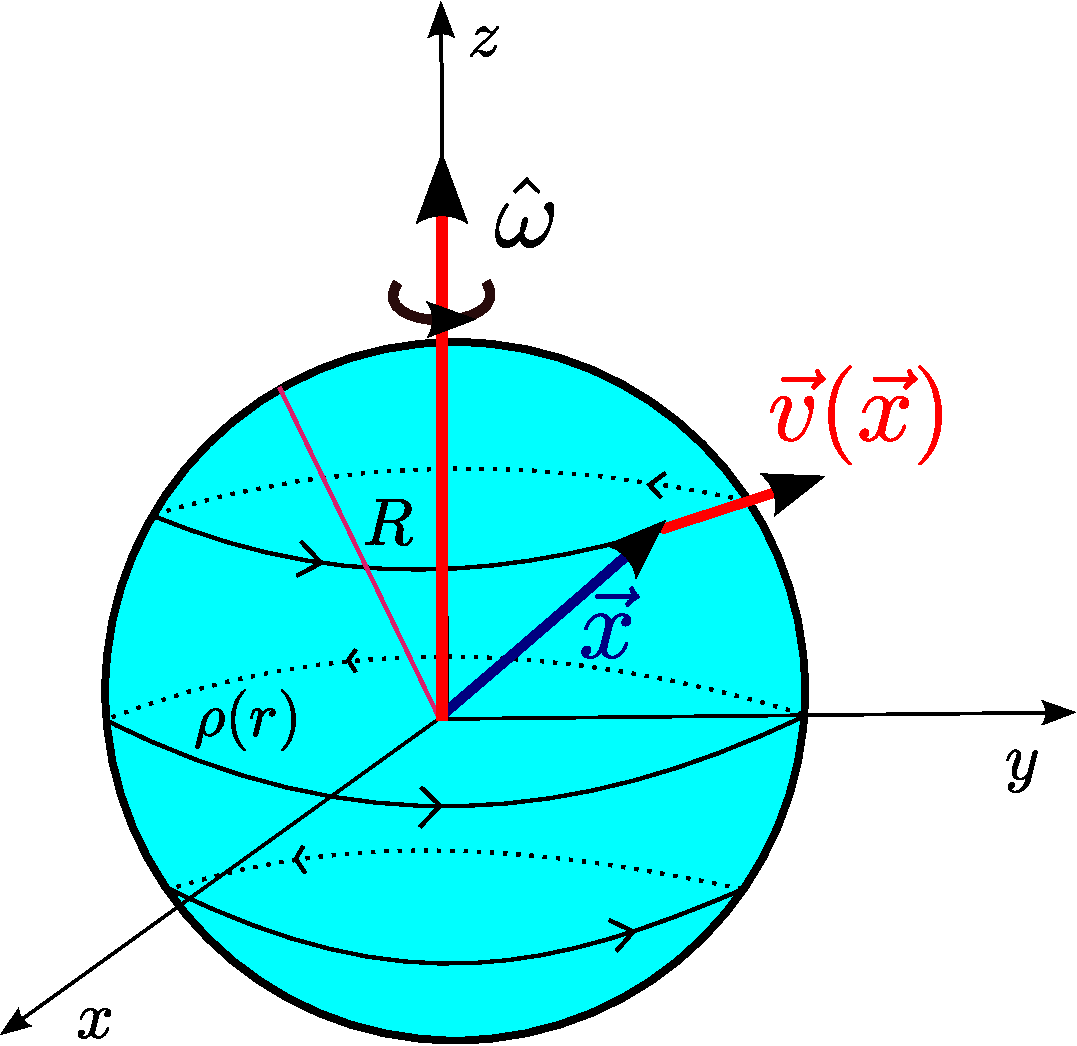
\includegraphics[angle=0,width=0.4\textwidth]{fig/fig-fuente.pdf}
\caption{Modelo de fuente de campo gravitacional: Una distribuci'on de masa esf'ericamente sim'etrica que rota, uniforme- y lentamente, en torno a un eje fijo.}
\label{fig:fuente}
\end{figure}

El campo de velocidades $\vec{v}(\vec{x})$ es entonces
\begin{align}
\vec{v}(\vec{x})={}&\vec{\omega}(r)\times\vec{x},
\end{align}
donde $\vec{\omega}=\omega(r)\hat{\omega}$ es la velocidad angular de la distribuci'on con respecto a la direcci'on fija $\hat{\omega}$. Suponemos que la rapidez angular $\omega(r)$ s'olo depende de la distancia radial $r$. El vector $\vec{x}$ puede ser escrito como
\begin{equation}
\vec{x}=r\, \hat{r}=r\left(\hat{\rho}\sen\theta +\hat{z}\cos\theta\right),
\end{equation}
con $\hat{\rho}=\hat{x}\cos\varphi+\hat{y}\sen\varphi$. Adem'as, podemos elegir la orientaci'on del sistema coordenado de modo que el eje de rotaci'on sea el eje $z$, es decir, $\hat{\omega}=\hat{z}$, con lo que $\vec{v}(\vec{x})$ se reduce a
\begin{align}
\vec{v}(\vec{x})={}&\omega(r)r(\hat{z}\times\hat{r})\\
 ={}&\omega(r)r\sen \theta (\hat{z}\times\hat{\rho})\\
 ={}&\omega(r)r\sen \theta\, \hat{\varphi} ,\label{campovelocidad}
\end{align}
donde $\hat{\varphi }=\hat{z}\times\hat{\rho}=-\hat{x}\sen\varphi +\hat{y}\cos\varphi $.

Ahora que ya tenemos una expresi'on general para el campo de velocidades de la distribuci'on, calculemos su mom'entum angular total $\vec{J}$, dado por
\begin{equation}
\vec{J}=\int_V \vec{x}\times(\rho \vec{v})\,d^3x.\label{mom'entumangular}
\end{equation}
Reemplazando (\ref{campovelocidad}) en (\ref{mom'entumangular}), podemos escribir
\begin{align}
\vec{J}={}&\int_V \rho (r)\omega(r)\sen \theta r^2(\hat{r}\times\hat{\varphi })d^3x\\
 ={}&\int_0^{2\pi}d\varphi \int_0^{\pi}d\theta \int_0^{R}dr\ \rho (r)\omega(r)\sen^2 \theta r^4\left(\sen \theta \hat{z}-\cos \theta \hat{\rho}\right)\\
 ={}&\hat{z}\int_0^{2\pi}d\varphi \int_0^{\pi}d\theta \sen^3 \theta  \int_0^{R}dr\ \rho (r)\omega(r)r^4\nonumber\\
 {}&-\int_0^{2\pi}d\varphi \ \hat{\rho}\int_0^{\pi}d\theta \sen^2 \theta \cos \theta  \int_0^{R}dr\ \rho (r)\omega(r)r^4.\label{j2}
\end{align}
Si adem'as reemplazamos las integrales $\int_0^{2\pi}\hat{\rho}\,d\varphi =\vec{0}$, $\int_0^{\pi}\sen^3\theta\,d\theta  ={4}/{3}$ en (\ref{j2}), obtenemos
\begin{equation}\boxed{
\vec{J}=\frac{8\pi}{3}\int_0^{R}\rho (r)\vec{\omega}(r)r^4\, dr.}\label{jgeneral}
\end{equation}

Calculemos ahora, a partir de la definici'on \eqref{defAret}, el potencial gravitomagn'etico $\vec{A}$ que produce esta distribuci'on de masa:
\begin{align}
\vec{A}(\vec{x})={}&-\frac{4G}{c}\int_V \frac{\rho (r') \vec{v}(\vec{x}')}{|\vec{x}-\vec{x}'|}\ d^3x'\\
 ={}&-\frac{4G}{c}\int_V \frac{\rho (r') \vec{\omega}(r')\times\vec{x}'}{|\vec{x}-\vec{x}'|}\ d^3x'\\
 ={}&-\frac{4G}{c}\int_0^{R}dr'r'^2\rho (r')\vec{\omega}(r')\times\left[\int_{\Omega}\frac{\vec{x}'}{|\vec{x}-\vec{x}'|}\ d\Omega'\right],\label{Aradialangular}
\end{align}
La integral angular en \eqref{Aradialangular} es conocida, y su valor es
\begin{equation}
\int_{\Omega}\frac{\vec{x}'}{|\vec{x}-\vec{x}'|}d\Omega'=
\dfrac{4\pi}{3}\frac{r'^2}{r^3}\, \vec{x}, \qquad r'<r .\label{intangular2}
\end{equation}
Reemplazando (\ref{intangular2}) en (\ref{Aradialangular}), obtenemos
\begin{align}
\vec{A}(\vec{x})={}&-\frac{16\pi G}{3cr^3}\int_0^{R}dr'r'^4\rho (r')\vec{\omega}(r')\times\vec{x}\\
={}&\frac{16\pi G}{3cr^3}\ \vec{x}\times\int_0^{R}dr'r'^4\rho (r')\vec{\omega}(r').\label{Acasi}
\end{align}

La integral en (\ref{Acasi}) es proporcional al mom'entum angular total $\vec{J}$ de la distribuci'on, dado por \eqref{jgeneral}. De este modo encontramos una expresi'on para el potencial gravitomagn'etico $\vec{A}(\vec{x})$ en t'erminos del mom'entum angular $\vec{J}$:
\begin{equation}\boxed{
\vec{A}(\vec{x})=-\frac{2G}{c}\ \frac{\vec{J}\times\vec{x}}{r^3},\qquad r>R.}\label{Afinal}
\end{equation}
Note que esta expresi'on tiene la misma forma (salvo factores que involucran las constantes gravitacionales y electromagn'eticas) que el potencial vectorial electromagn'etico producido por un \textit{dipolo magn'etico} (ideal) con momento dipolar magn'etico $\vec{\mu}$.

Calculando el rotor de \eqref{Afinal} obtenemos la expresi'on final para el campo gravitomagn'etico estacionario, producido por la esfera rotante con mom'entum angular constante $\vec{J}$:
\begin{equation}\boxed{
\vec{H}(\vec{x})=-\frac{2G}{c}\ \frac{3(\vec{J}\cdot\hat{r})\hat{r}-\vec{J}}{r^3},\qquad r>R.}\label{Hgravito}
\end{equation}

Por otro lado, el potencial gravitoel'ectrico estacionario producido por la distribuci'on de masa continua siendo el newtoniano, es decir,
\begin{equation}\boxed{
\phi(\vec{x})=-\frac{GM}{r},\qquad r>R,}\label{phifinal}
\end{equation}
donde $M$ es la masa total de la distribuci'on definida como es usual por,
\begin{equation}
M:=\int_V \rho (\vec{x})\, d^3x,\label{masatotal}
\end{equation}

Finalmente, el campo gravitoel'ectrico, de acuerdo a \eqref{cge}, es
\begin{equation}\boxed{
\vec{g}(\vec{x})=-\frac{GM}{r^2}\hat{r},\qquad r>R.}\label{ggravito}
\end{equation}

Pensando en la analog'ia con la electrodin'amica, este resultado es id'entico en forma al campo electroest'atico producido por una distribuci'on de carga esf'ericamente sim'etrica con carga total $Q$.

En la figura \ref{fig:gravitoelectromagnetico} podemos ver un esquema de las l'ineas de campo gravitoel'ectrico y gravitomagn'etico que produce la distribuci'on de masa rotante. Esta fuente de campo se caracteriza completamente por su mom'entum angular total $\vec{J}$ y por su masa total $M$.
\begin{figure}[H]
\centering
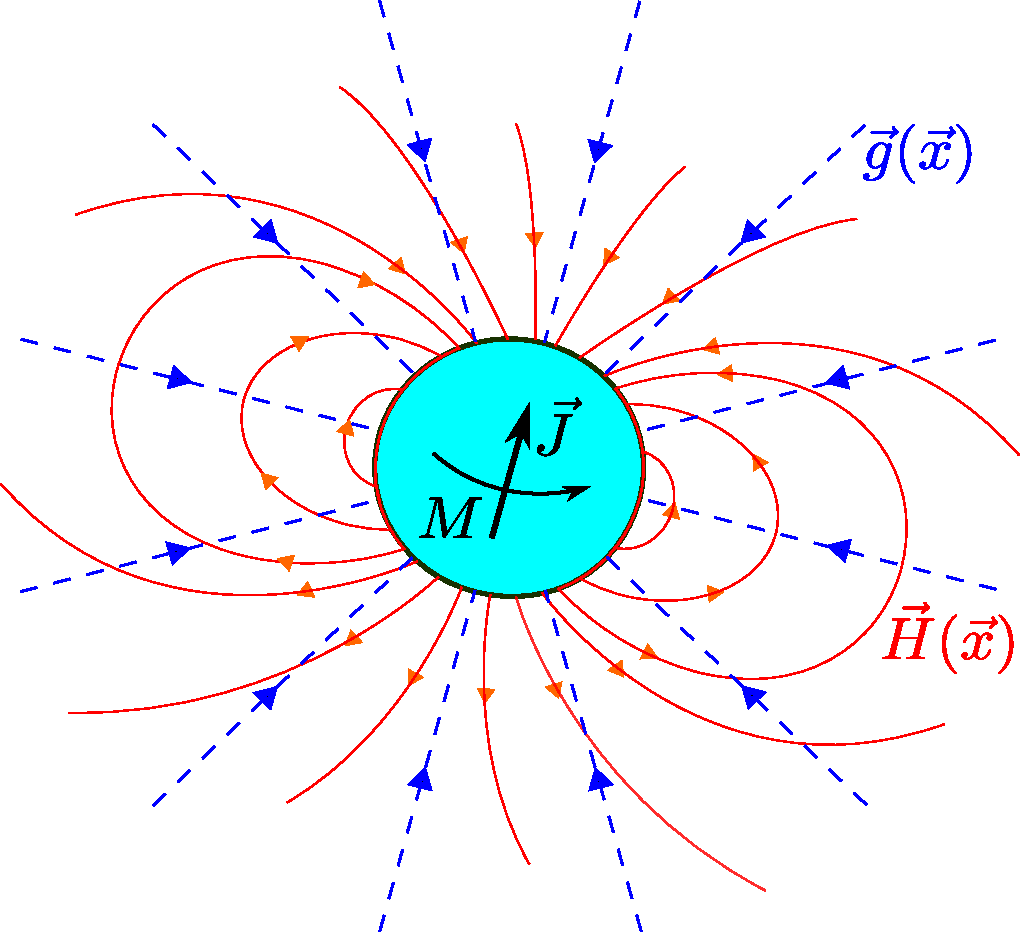
\includegraphics[angle=0,width=0.5\textwidth]{fig/fig-gravitoelectromagnetico.pdf}
\caption{L'ineas de campo gravitoel'ectrico y gravitomagn'etico, producidas por una distribuci'on esf'ericamente sim'etrica de masa total $M$ y que rota con mom'entum angular total constante $\vec{J}$.}
\label{fig:gravitoelectromagnetico}
\end{figure}

Note que las l'ineas de campo gravitomagn'etico mostradas en \ref{fig:gravitoelectromagnetico} tienen sentido opuesto al del campo magn'etico generado por una distribuci'on rotante de carga (positiva). Esto se suma al conocido hecho que las l'ineas de campo gravitoel'ectrico tienen sentido opuesto a las del campo el'ectrico producido por cargas positivas.

Para finalizar el an'alisis de esta secci'on, comparemos los 'ordenes de magnitud de los campos $\vec{g}$ y $\vec{H}$, producidos por la esfera rotante. De las expresiones (\ref{Hgravito}) y (\ref{ggravito}), podemos ver que estos campos son del orden,
\begin{equation}\label{magg}
g\sim \frac{GM}{R^2}, \qquad H\sim \frac{GJ}{cR^3}.
\end{equation}
Para estimar el orden de magnitud de $J$ podemos hacer $J\sim I\omega\sim MvR$, con lo que obtenemos
\begin{equation}
\frac{H}{g}\sim\frac{v}{c}\ll 1.
\end{equation}

Vemos que, debido a las velocidades no-relativistas de la fuente, el campo gravitomagn'etico producido es mucho menor en magnitud el correspondiente campo gravitoel'ectrico. Por ejemplo, para el Sol y la Tierra $v/c\sim10^{-6}$, por lo que en estos casos $\vec{H}$ es al menos seis 'ordenes de magnitud menor que $\vec{g}$.

\subsection{Geometr'ia del espaciotiempo fuera de la distribuci'on de masa esf'erica rotante}

Retornando a la descripci'on geom'etrica de la teor'ia, podemos determinar la m'etrica  y el elemento de l'inea del espaciotiempo fuera de la distribuci'on esf'erica rotante, en t'erminos de los par'ametros que caracterizan a la fuente: su masa total $M$ y su mom'entum angular total $\vec{J}$.

El eje fijo de rotaci'on de la distribuci'on rompe la simetr'ia esf'erica que tendr'ia el espaciotiempo si la fuente estuviese est'atica. Sin embargo, persiste una simetr'ia axial remanente  en torno a la direcci'on definida por el eje de rotaci'on del cuerpo. Sin p'erdida de generalidad, podemos elegir un sistema coordenado en que el eje de rotaci'on del cuerpo coincida con el eje $z$, de tal forma que el mom'entum angular de la distribuci'on se pueda expresar en la forma,
\begin{equation}
\vec{J}=J\hat{z}.
\end{equation}
En este caso, se tiene que los potenciales $\phi$ y $\vec{A}$ toman una forma m'as simple,
\begin{equation}
\phi(r) = -\frac{GM}{r},\label{phiii}\\
\end{equation}
\begin{equation}
\vec{A}(r,\theta,\varphi ) = -\frac{2GJ}{c}\frac{\hat{z}\times\hat{r}}{r^2}
=-\frac{2GJ}{c}\frac{\sen \theta }{r^2}\hat{\varphi}%=-\frac{2GJ}{c}\frac{\sen \theta }{r^2}\left[-\hat{x}\sen\varphi +\hat{y}\cos\varphi\right]
.\label{aphii}
\end{equation}
Si reemplazamos ahora \eqref{aphii} en \eqref{ds2phiA}, obtenemos el elemento de l'inea:
%\begin{equation}
%g_{\mu\nu}(x):=
%\left( \begin{array}{cccc}
%\vspace{4mm}
%1-\frac{2GM}{c^2r} & -\frac{2GJ}{c^3r^2}\sen \theta \sen\varphi & \frac{2GJ}{c^3r^2}\sen \theta \cos\varphi & 0 \\
%\vspace{4mm}
%-\frac{2GJ}{c^3r^2}\sen \theta \sen\varphi &-1-\frac{2GM}{c^2r} & 0 & 0 \\
%\vspace{4mm}
%\frac{2GJ}{c^3r^2}\sen \theta \cos\varphi & 0 &-1-\frac{2GM}{c^2r} & 0 \\
%0 & 0 & 0 &-1-\frac{2GM}{c^2r} \\
%\end{array} \right)+\mathcal{O}(G^2).\label{grafica2}
%\end{equation}
\begin{equation}
ds^2=\left(1-\frac{2GM}{c^2r}\right)c^2dt^2-\left(1+\frac{2GM}{c^2r}\right)d\vec{x}^2+\frac{4GJ}{c^3r^2}\sen\theta (\hat\varphi\cdot d\vec{x})cdt+\mathcal{O}(G^2).\label{ds22}
\end{equation}
En coodenadas esf'ericas, sabemos que $\hat\varphi\cdot d\vec{x}=r\sen\theta\,d\varphi$, y por lo tanto la expresi'on a primer orden en $G$ para el elemento de l'inea fuera de la distribuci'on esf'erica rotante, en coordenadas esf'ericas y en t'erminos de $M$ y $J$, resulta ser
\begin{equation}\boxed{
ds^2=\left(1-\frac{2GM}{c^2r}\right)c^2dt^2-\left(1+\frac{2GM}{c^2r}\right)\left[dr^2+r^2d\Omega^2\right]+\frac{4GJ}{c^3r}\sen^2 \theta d\varphi (cdt)+\mathcal{O}(G^2).}\label{dssss2}
\end{equation}
Es posible verificar que la soluci'on exacta del agujero negro rotante de Kerr en coordenadas isotr'opicas, se reduce a (\ref{dssss2}) en el l'imite de campo debil. Si adicionalmente hacemos $J=0$ recobramos la soluci'on de Schwarzschild, a primer orden en $G$, tambi'en en coordenadas isotr'opicas.

\section{Estudio de 'orbitas y resoluci'on perturbativa de la ecuaci'on del movimiento para una part'icula ligada y no-relativista en el espaciotiempo fuera de una esfera rotante.}

\section{Precesi'on Relativista de Gir'oscopos}

Una de las formas de testear las predicciones de RG respecto al campo gravitomagn'etico, es describiendo los efectos que la presencia de 'este campo produce sobre \textit{peque\~nos cuerpos de prueba con movimiento interno de rotaci'on} (``spin"), es decir, sobre lo que llamaremos un \textit{gir'oscopo}.

\subsection{Gir'oscopos y 4-vector de spin}

Modelamos un gir'oscopo como un peque\~no cuerpo caracterizado no s'olo por %su masa $m$, 
su posici'on $\vec{x}(t)$ y su velocidad $\vec{v}(t)$, sino que adem'as por un \textit{vector de mom'entum angular de rotaci'on propia} o \textit{spin} $\vec{S}(t)$, que describe la rotaci'on en torno a su propio eje. En la pr'actica se construyen gir'oscopos mec'anicos y 'opticos (ver \cite{1} para m'as detalles.)
%El mom'entum lineal del cuerpo se define como es usual:
%\begin{align}
%\vec{p}:=m\vec{v}
%\end{align}
%y su mom'entum angular orbital por
%\begin{align}
%\vec{L}:=\vec{x}\times\vec{p}.
%\end{align}

La propiedad b'asica de un gir'oscopo, es que \textit{en ausencia de fuerzas y torques externos ellos mantienen constante la magnitud y direcci'on de su spin $\vec{S}$}, respecto a un SRI, es decir, 
\begin{align}
\frac{d\vec{S}}{dt}=\vec{0}.\label{dinamicaS1}
\end{align}


Como sabemos, para describir el movimiento de un cuerpo en la Teor'ia Especial de la Relatividad, es 'util parametrizar las cantidades usando el tiempo propio $\tau$ y definir la 4-posici'on del objeto $x^\mu (\tau)$, adem'as de su 4-velocidad $u^\mu (\tau)$. Por otro lado, para describir el vector de spin $\vec{S}$, definimos un \textit{4-vector de spin} $S^\mu (\tau)$, tal que en el SRI com'ovil con el gir'oscopo s'olo tiene componentes espaciales:
\begin{align}
S^\mu \stackrel{*}{=}(0,\vec{S}).
\end{align}
Puesto que en este SRI la 4-velocidad del cuerpo es dada por $u^\mu\stackrel{*}{=}(u^0,\vec{0})$, entonces se tiene $S^\mu u_\mu\stackrel{*}{=}0$. Como consecuencia $S^{\mu}$ es ortogonal a $u^{\mu}$ en todo SRI, ya que $S^\mu u_\mu$ es un escalar:
\begin{equation}\boxed{\label{escalarSu2}
S^\mu u_\mu=0.}
\end{equation}

Adem'as, como la 4-velocidad del gir'oscopo es un 4-vector tipo tiempo, es decir $u^{\mu}u_{\mu}>0$, entonces de (\ref{escalarSu2}) se desprende que $S^{\mu}$ es siempre un vector tipo espacio, es decir, $S^\mu S_{\mu}<0$.

As'i, en Relatividad Especial, un gir'oscopo ser'a descrito por 
%su masa $m$, 
su 4-posici'on $x^{\mu}(\tau)$, su 4-velocidad $u^{\mu}(\tau)$ y su vector de spin $S^{\mu}(\tau)$, tal como se ilustra en la figura \ref{giroscopo}. La ecuaci'on que describe la din'amica de $S^{\mu}$, en ausencia de fuerzas y torques externos, se debe reducir a (\ref{dinamicaS1}), y es dada en cualquier SRI por
\begin{equation}\boxed{
\frac{dS^{\mu}}{d\tau}=0.}\label{dinamicaS2}
\end{equation}
\begin{figure}[H]
\centering
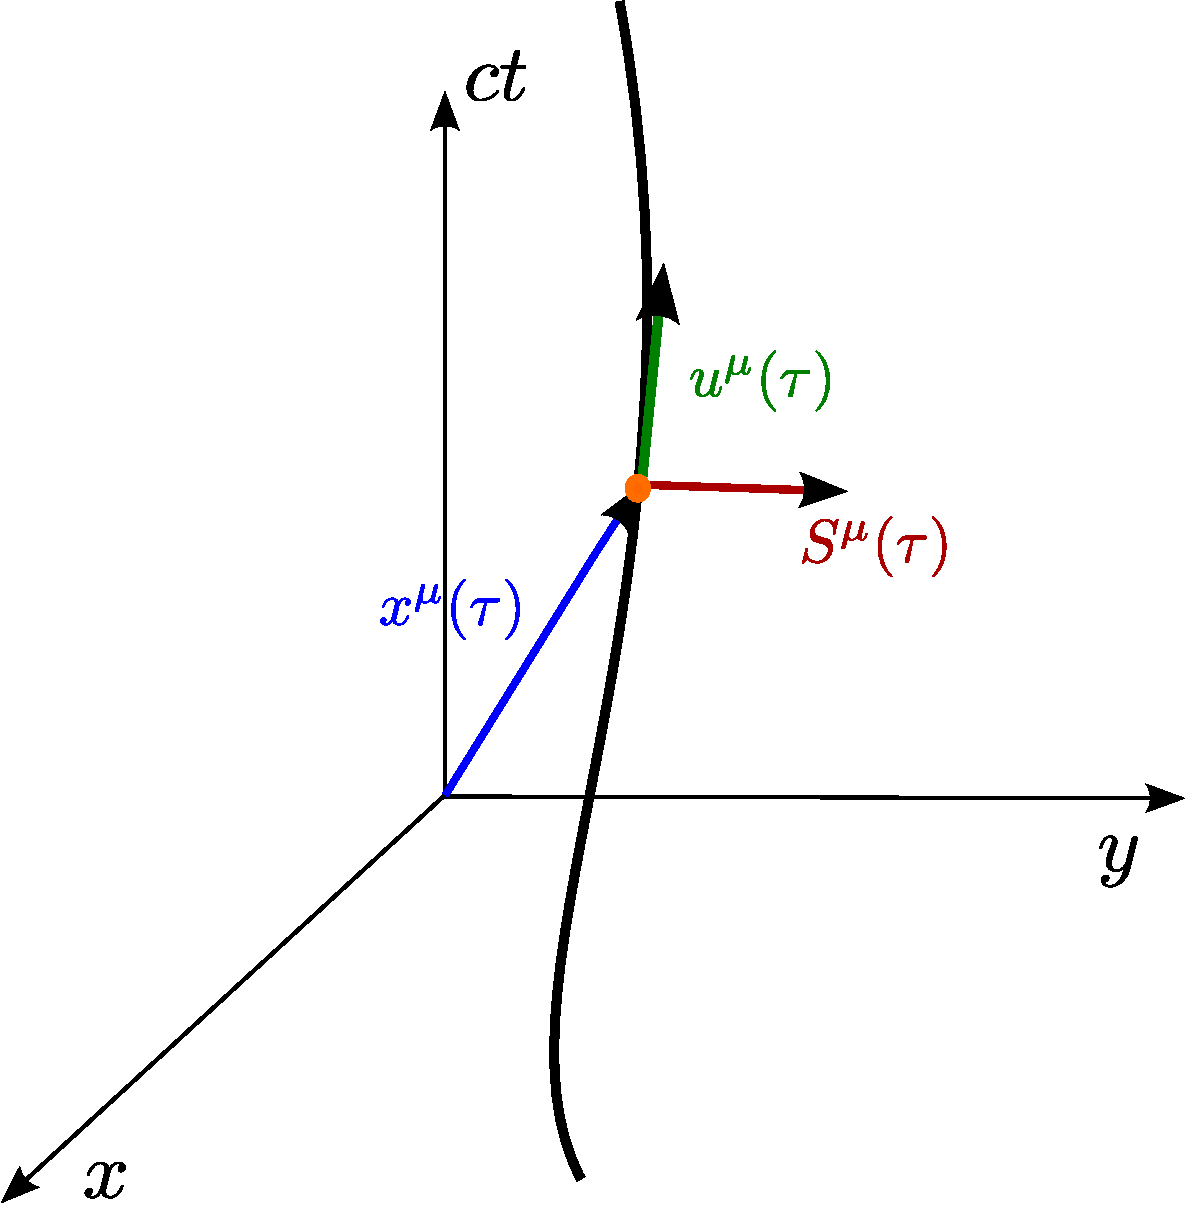
\includegraphics[angle=0,width=0.4\textwidth]{fig/fig-giroscopo.pdf}
\caption{Un gir'oscopo.}
\label{giroscopo}
\end{figure}

\subsection{Determinaci'on de la velocidad angular de precesi'on del spin de un gir'oscopo movi'endose en una geod'esica bajo la acci'on del campo gravitomagn'etico.}

Consideremos un gir'oscopo que se mueve en el espaciotiempo fuera de una fuente de campo gravitacional, con 4-velocidad
\begin{equation}
u^\mu (\tau):=\frac{dx^\mu }{d\tau}.
\end{equation}
Requerimos una ecuaci'on de evoluci'on para el vector $S^\mu$ en un campo gravitacional no nulo. Para encontrarla, hacemos uso del principio de equivalencia de Einstein. En ausencia de gravitaci'on (y adem'as de fuerzas y torques netos de otras fuerzas), la direcci'on y magnitud del vector de spin es constante respecto a un SRI. Por lo tanto, lo mismo debe ocurrir, de acuerdo a este principio, en un SRLI. Si $\bar{x}^\mu$ son las coordenadas geod'esicas asociadas a un SRLI, entonces (ver \eqref{dinamicaS2}): 
\begin{equation}\label{dSdtauast0}
\frac{d\bar{S}^\mu }{d\tau}\stackrel{*}{=}0.
\end{equation}
En coordenadas arbitrarias, tendremos
\begin{equation}\label{fwt}
\boxed{\frac{DS^\mu }{D\tau}=0,}
\end{equation}
donde hemos introducido la \textit{derivada covariante a lo largo de la l'inea de mundo $x^\mu(\tau)$}:
\begin{equation}\label{DSDtau}
\frac{DS^\mu}{D\tau}:=\frac{dS^\mu}{d\tau}+\Gamma^{\mu}_{\ \nu\lambda}S^\nu u^\lambda .
\end{equation}
Claramente, la ecuaci'on \eqref{fwt} se reduce a \eqref{dSdtauast0} en coordenadas geod'esicas, ya que las componentes de la conexi'on se anulan\footnote{Note que este resultado es v'alido para \textit{todo evento sobre la l'inea de mundo} $x^\mu(\tau)$.}. Adem'as, \eqref{DSDtau} es un vector bajo TGC's. Esto puede verificarse f'acilmente notando que podemos escribir
\begin{equation}
\frac{DS^\mu}{D\tau}:=u^\nu\nabla_\nu S^\mu,
\end{equation}
que es la generalizaci'on covariante de la derivada respecto al tiempo propio $\tau$ (que mide un observador com'ovil con el gir'oscopo) a lo largo de la trayectoria $x^\mu (\tau)$:
\begin{equation}
\frac{dS^\mu }{d\tau}=u^{\nu}\partial_{\nu} S^{\mu}.
\end{equation}
%Cualquier 4-vector que satisfaga una ecuaci'on de la forma de (\ref{fwt}), se dice que efect'ua un transporte de ``Fermi-Walker'' a lo largo de su trayectoria.

Si contraemos la ecuaci'on (\ref{fwt}) con $S_{\mu}$, completamos la derivada covariante total, parametrizada con respecto a $\tau$, y usamos el hecho que para un escalar la derivada covariante coincide con la derivada parcial, se encuentra que $S^\mu S_{\mu}$ es una \textit{constante del movimiento}, es decir,
\begin{equation}\boxed{
\frac{d\ }{d\tau}\left(S^\mu S_{\mu}\right)=0.}\label{SSconstante}
\end{equation}

En particular, consideremos el caso de un gir'oscopo que orbita (dentro de un sat'elite) una fuente de campo gravitacional (la Tierra, por ejemplo). Supongamos que el sat'elite est'a construido de tal forma que es capaz de proteger al gir'oscopo de toda influencia externa no-gravitacional, haciendo que su 4-aceleraci'on $a^\mu $ sea nula y por consiguiente el gir'oscopo se mueva en una geod'esica bajo la acci'on del campo gravitacional,
\begin{equation}
a^\mu (\tau):=\frac{d^2x^\mu }{d\tau^2}+\Gamma^\mu _{\ \nu\lambda}\frac{dx^{\nu}}{d\tau}\frac{dx^{\lambda}}{d\tau}=0.
\end{equation}
Bajo estas consideraciones,  las ecuaciones (\ref{fwt}) y (\ref{SSconstante}) son v'alidas para describir la din'amica del 4-vector de spin $S^{\mu}(\tau)$.

En la figura \ref{GPB} se muestra gr'aficamente el problema que queremos analizar para el caso particular de un gir'oscopo dentro de un sat'elite que orbita la Tierra, como es el caso del proyecto GPB.
\begin{figure}[H]
\centering
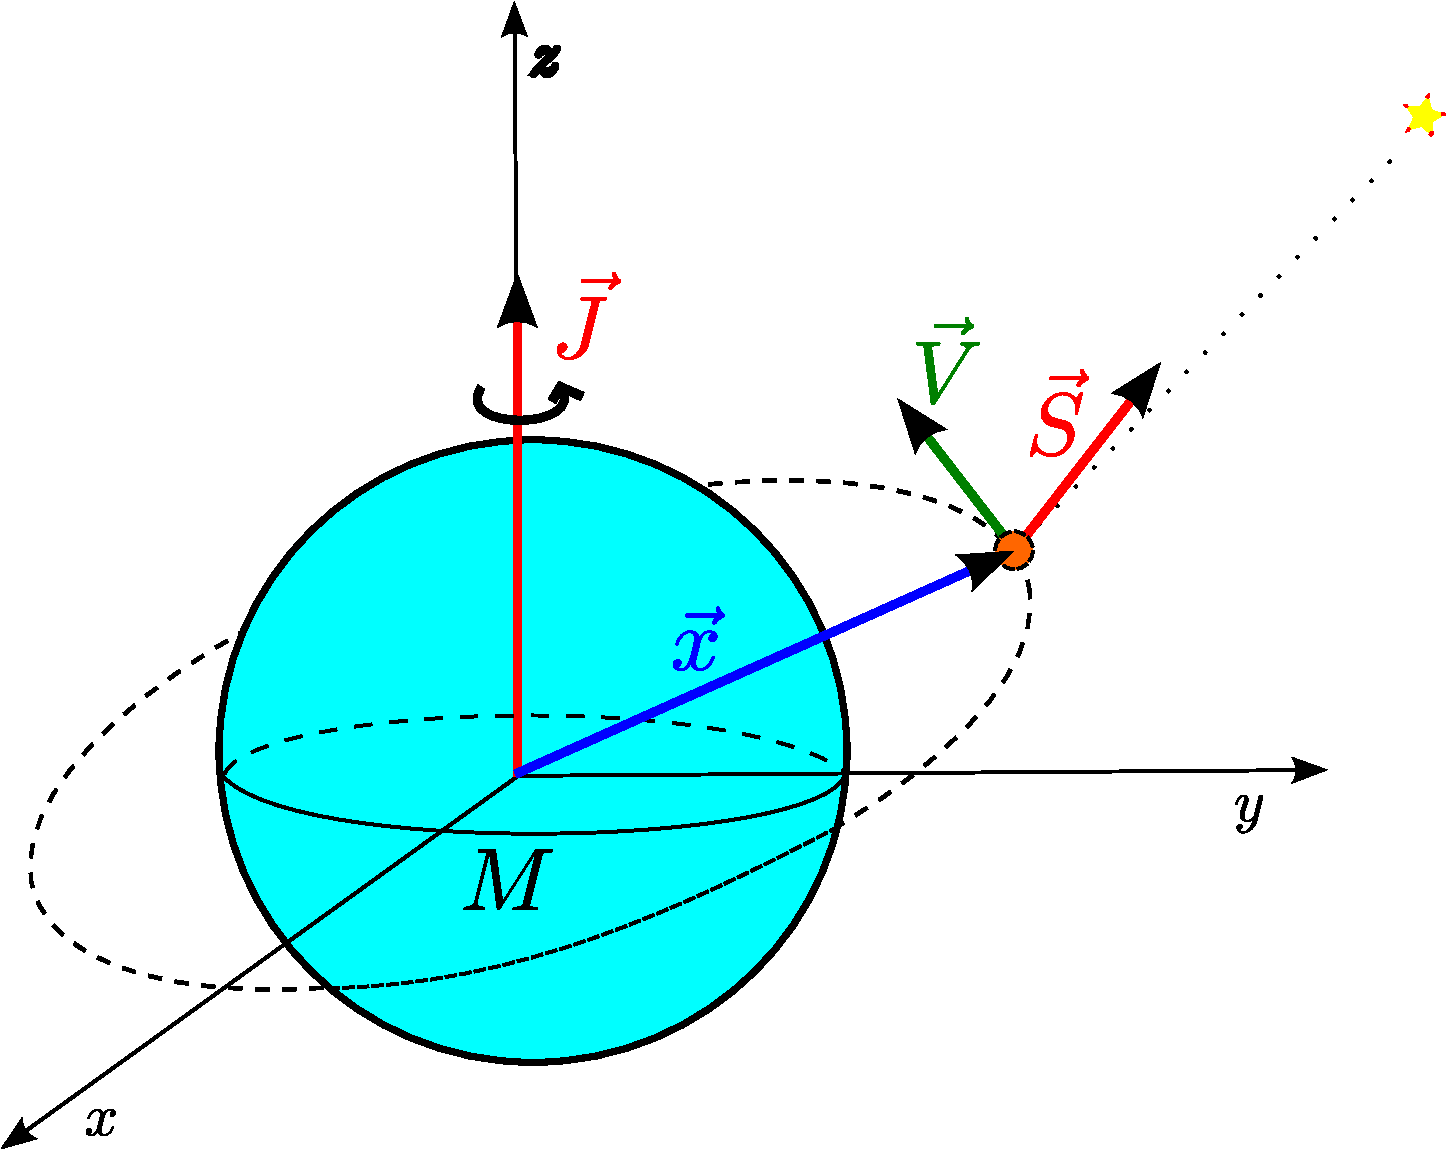
\includegraphics[angle=0,width=0.5\textwidth]{fig/fig-GPB.pdf}
\caption{Gir'oscopo que describe una geod'esica en torno a la Tierra.}
\label{GPB}
\end{figure}
Ahora expresamos las derivadas en \eqref{escalarSu2}, \eqref{fwt} con \eqref{DSDtau} y  \eqref{SSconstante} en t'erminos de la coordenada temporal $t$ del observador cuasi-inercial, con lo que obtenemos 
\begin{align}
\frac{dS^\mu }{dt}+\Gamma^\mu _{\ \nu\lambda}S^{\nu}\frac{dx^{\lambda}}{dt}={}&0,\label{giro1}\\
g_{\mu\nu}S^\mu S^{\nu}={}&\text{cte},\label{giro2}\\
g_{\mu\nu}S^\mu \frac{dx^{\nu}}{dt}={}&0.\label{giro3}
\end{align}
El paso siguiente es calcular las ecuaciones \eqref{giro1}-\eqref{giro3}, consistentemente hasta orden $G^{3/2}$, reescribi'endolas en t'erminos de la velocidad $v^i=dx^i/dt$ del gir'oscopo, el vector de spin $S^i$ (componentes espaciales) y los potenciales $\phi$ y $A^i$.

Primero, si evaluamos (\ref{giro1}) para $\mu=i$ y notamos que $dx^{0}/dt=c$, encontramos
\begin{equation}
\frac{dS^{i}}{dt}+c\Gamma^{i}_{\ 00}S^{0}+\Gamma^{i}_{\ 0j}S^{0}v^j+c\Gamma^{i}_{\ j0}S^{j}+\Gamma^{i}_{\ jk}S^{j}v^k=0.\label{giro12}
\end{equation}
Luego, si reemplazamos en (\ref{giro12}), los valores de los s'imbolos de Christoffel dados en (\ref{simbolo1})-(\ref{simbolo6}), obtenemos
\begin{align}
\frac{dS^{i}}{dt}={}&-\frac{1}{c}(\partial_i\phi)S^0+\frac{1}{2c^2}(\partial_i A^j-\partial_j A^i)S^0v^j+\frac{1}{c^3}\frac{\partial \phi}{\partial t}S^0v^i+\frac{1}{2c}(\partial_i A^j-\partial_j A^i)S^j+\frac{1}{c^2}\frac{\partial \phi}{\partial t}S^i\nonumber\\
{}&-\frac{1}{c^2}(\partial_i \phi) S^jv^j+\frac{1}{c^2}v^j(\partial_j\phi)S^i+\frac{1}{c^2}(\partial_j \phi) S^jv^i+\mathcal{O}(G^2)\label{dsidt}.
\end{align}

%Por otra parte, usando las expresiones para las componentes de la m'etrica $g_{\mu\nu}$ en t'erminos de los potenciales, dadas en (\ref{gphiA}), podemos escribir expl'icitamente (\ref{giro2}) hasta orden $G$:
%\begin{equation}
%(S^0)^2+\frac{2}{c^2}\phi(S^0)^2-\frac{2}{c^2}A^iS^0S^i-S^iS^i+\frac{2}{c^2}\phi S^iS^i+\mathcal{O}(G^2)=\text{cte}.\label{sisicte}
%\end{equation}
Necesitamos escribir $S^0$ en t'erminos de las dem'as cantidades, para lo cual la ecuaci'on (\ref{giro3}) nos ser'a 'util:
\begin{align}
S^0-\frac{2\phi}{c^2}S^0-\frac{1}{c^3}A^iv^iS^0-\frac{1}{c^2}A^iS^i-\frac{1}{c}S^iv^i-\frac{2\phi}{c^3}S^iv^i+\mathcal{O}(G^2)=0.\label{giro32}
\end{align}
De \eqref{giro32} podemos despejar $S^0$, como siempre despreciando t'erminos de orden $G^2$:
\begin{equation}
S^0=\frac{1}{c}v^iS^i+\frac{1}{c^2}A^iS^i+\frac{4}{c^3}\phi S^iv^i+\mathcal{O}(G^2).\label{S00}
\end{equation}
Note que el t'ermino $(S^iv^i)(A^jv^j)/c^4$ ha sido despreciado debido a que es de orden $G^2$, pues $v^i\sim G^{1/2}$. 
%A partir de \eqref{S00} calculamos $(S^0)^2$ qued'andonos con t'erminos hasta orden $G^{3/2}$:
%\begin{equation}
%(S^0)^2=\frac{1}{c^2}(v^iS^i)(v^jS^j)+\frac{2}{c^3}(A^iS^i)(v^jS^j)+\mathcal{O}(G^2).\label{S002}
%\end{equation}
Finalmente, si reemplazamos \eqref{S00} %y \eqref{S002} 
en \eqref{dsidt}, %y \eqref{sisicte}
obtenemos dos ecuaciones en que s'olo aparecen $S^i$, $v^i$, $\phi$ y $A^i$, dadas por
\begin{align}
\frac{dS^{i}}{dt} &= \frac{1}{2c}\left(\partial_iA^j-\partial_jA^i\right)S^j+\frac{1}{c^2}\frac{\partial \phi}{\partial t}S^i \nonumber \\
&\quad  -\frac{2}{c^2}(\partial_i\phi) S^jv^j+\frac{1}{c^2}(\partial_j\phi)v^jS^i+\frac{1}{c^2}(\partial_j\phi)S^jv^i+\mathcal{O}(G^2).\label{dsidt2}
\end{align}
%\begin{equation}
%S^iS^i-\frac{2\phi}{c^2}S^iS^i-\frac{1}{c^2}(v^iS^i)^2+\mathcal{O}(G^2)=\text{cte}.\label{sisicte2}
%\end{equation}
%La ecuaci'on (\ref{sisicte2}) sugiere definir el vector de spin auxiliar 
%\begin{equation}\boxed{
%{\cal L}^i:=\left(1-\frac{1}{c^2}\phi\right)S^i-\frac{1}{2c^2}v^i(v^jS^j),}\label{defli}
%\end{equation}
%cuyo m'odulo cuadrado reproduce precisamente el lado izquierdo de \eqref{sisicte2}, y por lo tanto satisface 
%\begin{equation}
%{\cal L}^i{\cal L}^i=\text{cte.}+\mathcal{O}(G^2) ,\label{lilicte}
%\end{equation}
%es decir, que su m'odulo cuadrado es constante a orden $G^{3/2}$.
%
%Expresamos ahora la ecuaci'on \eqref{dsidt2} en t'erminos de la variable auxiliar ${\cal L}^i$. Para ello, calculamos su derivada temporal a partir de su definici'on en \eqref{defli}:
%\begin{equation}
%\frac{d{\cal L}^i}{dt}=-\frac{1}{c^2}\frac{\partial\phi}{\partial t}S^i-\frac{1}{c^2}v^j(\partial_j\phi)S^i+\frac{dS^i}{dt}-\frac{\phi}{c^2}\frac{dS^i}{dt}-\frac{1}{2c^2}v^jS^j\frac{dv^i}{dt}-\frac{1}{2c^2}v^iS^j\frac{dv^j}{dt}-\frac{1}{2c^2}v^iv^j\frac{dS^j}{dt}.\label{dlidt}
%\end{equation}
%Luego, reemplazando (\ref{dsidt2}) y la ecuaci'on del movimiento (\ref{movnorel}) en (\ref{dlidt}), se obtiene la siguiente ecuaci'on que incluye t'erminos hasta  orden $G^{3/2}$:
%\begin{align}
%\frac{d{\cal L}^i}{dt}=\frac{1}{2c}(\partial_iA^j-\partial_jA^i)S^j+\frac{3}{2c^2}\left(v^i\partial_j\phi-v^j\partial_i\phi\right)S^j+\mathcal{O}(G^2).\label{dlidt2}
%\end{align}
%Finalmente, podemos reemplazar $S^j$ por ${\cal L}^j$ en el lado derecho de (\ref{dlidt2}), ya que ambas cantidades difieren en t'erminos de orden mayor o igual a $G$. Adem'as, si utilizamos el s'imbolo de Levi-Civita, obtenemos
%\begin{equation}
%\frac{d{\cal L}^i}{dt}=\frac{1}{2c}\epsilon_{ijk}{\cal L}^j\left(\epsilon_{klm}\partial_l A^m\right)+\frac{3}{2c^2}\epsilon_{ijk}{\cal L}^k\left(\epsilon_{jlm}v^l\partial_m\phi\right)+\mathcal{O}(G^2),\label{dlidt3}
%\end{equation}
%y en notaci'on vectorial,
%\begin{equation}\boxed{
%\frac{d\vec{{\cal L}}}{dt}=\left[-\frac{1}{2c}(\vec{\nabla}\times\vec{A})-\frac{3}{2c^2}(\vec{v}\times\vec{\nabla}\phi)\right]\times\vec{{\cal L}}+\mathcal{O}(G^2).}
%\end{equation}
Esta ecuaci'on puede reescribirse como 
\begin{align}
\frac{dS^i}{dt} =& \frac{1}{2c}\epsilon_{ijk}S^j\left(\epsilon_{klm}\partial_l A^m\right)+\frac{3}{2c^2}\epsilon_{ikj}S^k\left(\epsilon_{jlm}v^l\partial_m\phi\right)\nonumber\\
& +\frac{1}{2c^2}\left[2(\partial_j\phi)v^jS^i-(\partial_i\phi)v^jS^j -(\partial_j\phi)v^iS^j\right]+\mathcal{O}(G^2),\label{dlidt3}
\end{align}
y en notaci'on vectorial,
\begin{equation}\boxed{
\frac{d\vec{S}}{dt} = \left[-\frac{1}{2c}(\vec{\nabla}\times\vec{A})-\frac{3}{2c^2}(\vec{v}\times\vec{\nabla}\phi)\right]\times\vec{S} 
+\frac{1}{2c^2}\left[2\vec{S}(\vec{v}\cdot\vec{\nabla}\phi)-(\vec{\nabla}\phi)\vec{v}\cdot\vec{S}
-(\vec{S}\cdot\vec\nabla\phi)\vec{v}\right]+\mathcal{O}(G^2).}
\end{equation}

%Debido a que adem'as $\vec{{\cal L}}$ en (\ref{lilicte}) satisface
%\begin{align}\boxed{
%\vec{{\cal L}}\hspace{1mm}^2+\mathcal{O}(G^2)=\text{cte},}
%\end{align}
%entonces podemos identificar una velocidad angular $\vec{\Omega}$ asociada a la precesi'on del spin auxiliar del gir'oscopo:
%\begin{equation}
%\frac{d\vec{{\cal L}}}{dt}=\vec{\Omega}\times\vec{{\cal L}}+\mathcal{O}(G^2),
%\end{equation}
\begin{equation}
\frac{d\vec{S}}{dt}=\vec{\Omega}\times\vec{{\cal S}}+\cdots + \mathcal{O}(G^2),
\end{equation}
donde hemos definido,
\begin{equation}
\vec{\Omega}:=\vec{\Omega}_{\rm GEO}+\vec{\Omega}_{\rm LT},
\end{equation}
con $\vec{\Omega}_{\rm GEO}$ la velocidad angular de preseci'on \emph{geod'esica}, dada por
\begin{align}\boxed{
\vec{\Omega}_{\rm GEO}:=\frac{3}{2c^2}(\vec{v}\times\vec{g}),}\label{geodetic}
\end{align}
y $\vec{\Omega}_{\rm LT}$ la velocidad angular de precesi'on de \emph{Lense-Thirring}, 
\begin{align}\boxed{
\vec{\Omega}_{\rm LT}:=-\frac{1}{2c}\vec{H},}\label{LT}
\end{align}
en honor a los dos cient'ificos que en 1918 predijeron este efecto conocido como ``frame-dragging''.


\subsection{Predicci'on de la teor'ia para un gir'oscopo que orbita la Tierra y que intenta medir el GPB}

Evaluemos las expresiones (\ref{geodetic}) y (\ref{LT}) para el caso de un gir'oscopo que orbita la Tierra, con lo que podremos obtener la famosa predicci'on que recientemente midi'o con 'exito el GPB \cite{Everitt11}. Usaremos los campos gravitoel'ectro y gravitomagn'etico, de una masa esf'ericamente sim'etrica rotando respecto a un eje fijo, calculados en (\ref{Hgravito}) y (\ref{ggravito}), de modo que en este caso
\begin{align}
\vec{g}(r)={}&-\frac{GM_T}{r^2}\hat{r},\label{gGPB}\\
\vec{H}(r)={}&-\frac{2GJ_T}{cr^3}\left[3(\hat{J}_T\cdot\hat{r})\hat{r}-\hat{J}_T\right]\label{BGPB},
\end{align}
donde $M_T$ es la masa total de la Tierra, $J_T$ su momento angular total y $\hat{J}_T$ el vector unitario la direcci'on de rotaci'on.

Por simplicidad, supongamos que el gir'oscopo gira en una \textit{'orbita circular} en torno a la Tierra, por lo que su velocidad se puede escribir en forma compacta por
\begin{equation}
\vec{v}=\left(\frac{M_TG}{R}\right)^{1/2}\hat{h}\times\hat{r},\label{aproxcirculo}
\end{equation}
donde $R$ es el radio de la 'orbita y $\hat{h}$ su vector unitario normal\footnote{Esta 'orbita circular es una geod'esica a primer orden en $G$. Ver por ejemplo \eqref{solucasi}.}. Ver la figura \ref{orbitaGPB}. Luego, reemplazando (\ref{gGPB}), (\ref{BGPB}) y (\ref{aproxcirculo}) en (\ref{geodetic}) y (\ref{LT}), obtenemos
\begin{align}
\vec{\Omega}_{\rm GEO}={}&\frac{3}{2c^2}\frac{M_T^{3/2}G^{3/2}}{R^{5/2}}\left[\hat{h}-(\hat{h}\cdot\hat{r})\hat{r}\right],\label{geo11}\\
\vec{\Omega}_{\rm LT}={}&\frac{GJ_T}{c^2R^3}\left[3(\hat{J}_T\cdot\hat{r})\hat{r}-\hat{J}_T\right].\label{LT11}
\end{align}
Consideremos adem'as el caso particular en que el gir'oscopo se mueve \textit{en una 'orbita polar alrededor de la Tierra}, es decir, tal que
\begin{align}
\hat{h}\cdot\hat{J}_T=0,
\end{align}
como se muestra en la figura \ref{orbitaGPB}.
\begin{figure}[H]
\centering
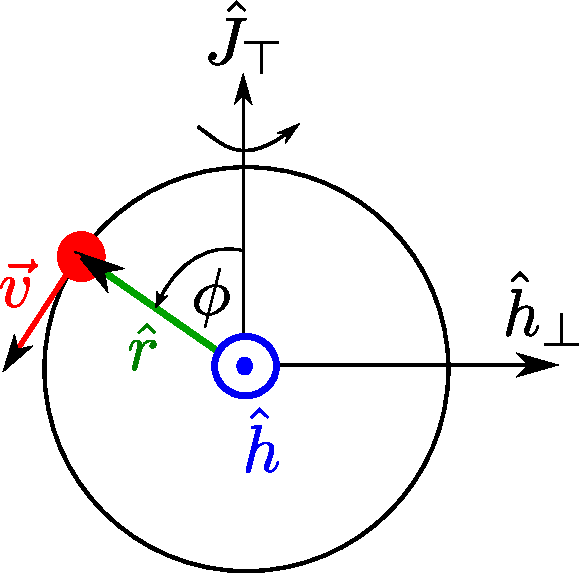
\includegraphics[angle=0,width=0.3\textwidth]{fig/fig-orbitaGPB.pdf}
\caption{Gir'oscopo en una 'orbita circular polar en torno a la Tierra.}
\label{orbitaGPB}
\end{figure}
De la figura vemos que podemos parametrizar la 'orbita por
\begin{align}
\hat{r}(\phi)=\hat{J}_T\cos\phi-\hat{h}_{\perp}\sen\phi,\label{parametrizacionorbita}
\end{align}
donde $\hat{h}_{\perp}$ es un vector unitario perpendicular a $\hat{h}$ y $\hat{J}_T$. Si reemplazamos (\ref{parametrizacionorbita}) en (\ref{geo11}) y (\ref{LT11}), y luego promediamos a lo largo de una 'orbita completa del gir'oscopo, es decir, $\phi\in[0,2)$, entonces las \emph{velocidades angulares promedio} de precesi'on por revoluci'on, quedan dadas finalmente por
\begin{equation}\boxed{
\begin{aligned}
\langle\vec{\Omega}_{\rm GEO}\rangle={}&\frac{3G^{3/2}}{2c^2}\frac{M_T^{3/2}}{R^{5/2}}\hat{h},\\
\langle\vec{\Omega}_{\rm LT}\rangle={}&\frac{G}{2c^2}\frac{J_T}{R^3}\hat{J}_T.\label{LT22}
\end{aligned}}
\end{equation}
Las expresiones (\ref{LT22}) son las predicciones de RG para el caso de un gir'oscopo orbitando una masa rotante en una 'orbita circular polar. Para obtener un resultado num'erico, consideramos a la Tierra como una esfera de radio $R_T=6,371\cdot 10^6{}m$ (***diferencia con tabla en ap'endice!***) y distribuci'on de masa esf'ericamente sim'etrica de masa total $M_T=5.97\cdot 10^{24}{}kg$. Sea la altura de la 'orbita polar circular de $642 km$ sobre la superficie de la Tierra, es decir, $h=6,42\cdot 10^5m$, por lo que se tiene $R=R_T+h=7,013\cdot 10^{6}m$. Para calcular el mom'entum angular total de rotaci'on de la Tierra, usamos su definici'on en (\ref{jgeneral}), con lo que obtenemos
\begin{align}
J_T=\frac{2}{5}M_TR_T^2\omega,
\end{align}
y finalmente considerando que el periodo de rotaci'on de la Tierra es $T=23.9345 hr$, se tiene $\omega=2\pi/T=7,2919\cdot 10^{-5}Hz$ y por consiguiente $J_T=7,0679\cdot 10^{33}kg\hspace{1mm}m^2/s$.
Luego, evaluando todos los datos en (\ref{LT22}), y considerando $G=6,67\cdot 10^{-11}N\hspace{1mm}m^2/kg^2$, las predicciones num'ericas de RG para la precesi'on del gir'oscopo que confirm'o el sat'elite GPB son:
\begin{align}
\langle\vec{\Omega}_{\rm GEO}\rangle={}&6.6\frac{sec}{yr}\hat{h},\\
\langle\vec{\Omega}_{\rm LT}\rangle={}&0.049\frac{sec}{yr}\hat{J}_T.
\end{align}

***No s'e por qu'e la precesi'on de Lense-Thirring difiere en $0.005 sec/yr$ con respecto al resultado de la figura 7.6 y en $0.007 sec/yr$ con respecto al paper oficial del GPB, que es $\langle\Omega_{\rm LT}\rangle=0.039 sec/yr$. El resultado experimental medido por GPB fue $\langle\Omega_{\rm LT}{}\rangle_{\rm\bf exp}=(0.0372\pm 0.0072) sec/yr$. Para m'as detalles ver \cite{Everitt11}. ***

\begin{figure}[H]
\centering
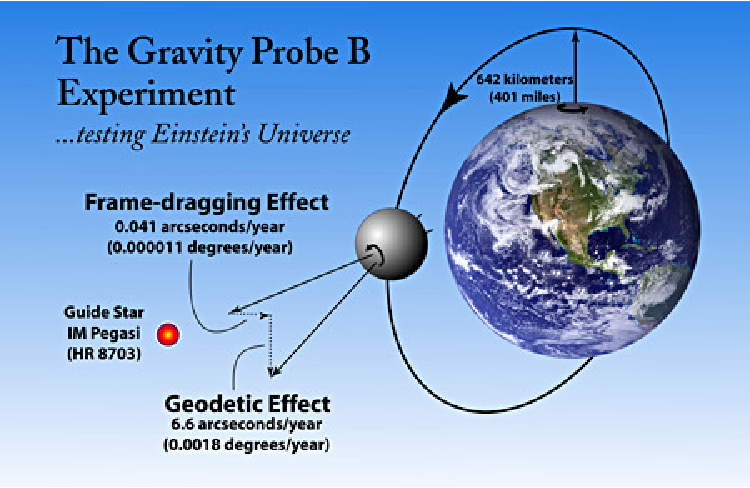
\includegraphics[angle=0,width=0.5\textwidth]{fig/fig-precesion.pdf}
\caption{Esquema de los 'angulos de precesi'on del gir'oscopo, medidos por la sonda GPB.}
\label{precesion}
\end{figure}